\documentclass[12pt]{article} 
\usepackage{pythonhighlight}

\usepackage[utf8]{inputenc}

% font types
\renewcommand{\familydefault}{\sfdefault}
% \usepackage{helvet}
% \usepackage[T1]{fontenc}
% \usepackage[utf8]{inputenc}

% package to rotate the page landscape 
%\usepackage[paper=portrait, pagesize]{typearea}
\usepackage[a4paper]{geometry}
\usepackage[usegeometry]{typearea}
%\usepackage[hmargin=.65in,vmargin=1.1in]{geometry}
%\usepackage[top=0.75in, left=0.75in, right=0.52in, bottom=1.44in]{geometry}

% only for dummy text
\usepackage{blindtext}
\usepackage{lipsum}
%\usepackage[margin=0.5in, left=0.5in, top=0.8in, includefoot]{geometry}
%\usepackage[a4paper, left=1.0in, right=1.0in, top=1.0in, bottom=1.0in]{geometry}

\usepackage[hidelinks]{hyperref} % Allows for clickable references

% Graphics preamble
\usepackage{graphicx} % import graphics package
%\graphicspath{ {/Users/tgol0003/Desktop/seagate4_2/uwgeo_models/production_models/} } % harddisk path
\usepackage{float} % Allows for control of float positions
\usepackage[section]{placeins} % to place figures in the section 
\usepackage{multicol} % position figures across the columns

% figures packages

% adding number with in section to equations
\usepackage{amsmath} 
\numberwithin{equation}{subsection} 
\makeatletter
\@addtoreset{equation}{section}
\makeatother

% Header and Footer info
\usepackage{fancyhdr}
\pagestyle{fancy}
\fancyhead{}
\fancyfoot{}
\fancyfoot[R]{\thepage}
\renewcommand{\headrulewidth}{0pt}
\renewcommand{\footrulewidth}{0pt}

\newgeometry{left=0.35in, right=0.35in, top=0.5in, bottom=1.0in}

\usepackage{changepage}

\begin{document} 

\cleardoublepage
\KOMAoptions{paper=portrait}
\recalctypearea
\newgeometry{left=0.1in, right=0.1in, top=0.1in, bottom=0.1in}

% \eject \pdfpagewidth=3in \pdfpageheight=10in % command to change the page height and width
\eject \pdfpagewidth=11.4in \pdfpageheight=10.8in 

\newpage

\vspace{1.5in} 

\textbf{Annulus Benchmark: Kramer etal}

\newpage

\textbf{Benchmark cases}
\vspace{0.2in}

\begin{adjustwidth}{1cm}{4cm}

\hspace{0.19in} Case1: Freeslip boundaries and delta function density perturbation 

Case2: Freeslip boundaries and smooth density distribution

Case3: Noslip boundaries and delta function density perturbation

Case4: Noslip boundaries and smooth density distribution 


\begin{python}
	# defining rho fn
	if delta_fn:
		rho = sympy.cos(n*th_uw) * sympy.exp(-1e5 * ((r_uw - r_int) ** 2))
		stokes.add_natural_bc(-rho * unit_rvec, "Internal")
	elif smooth:
		rho = ((r_uw/r_o)**k)*sympy.cos(n*th_uw)
	
	# boundary conditions
	if freeslip:
		if ana_normal:
			Gamma = mesh.CoordinateSystem.unit_e_0
		elif petsc_normal:
			Gamma = mesh.Gamma
	
		# Gamma = norm_v.sym
		stokes.add_natural_bc(2.5e3 * Gamma.dot(v_uw.sym) *  Gamma, "Upper")
		stokes.add_natural_bc(2.5e3 * Gamma.dot(v_uw.sym) *  Gamma, "Lower")
	
	elif noslip:
		stokes.add_essential_bc(sympy.Matrix([0., 0.]), "Upper")
		stokes.add_essential_bc(sympy.Matrix([0., 0.]), "Lower")
\end{python}
\end{adjustwidth}

\vspace{1.2in}
\textbf{Mesh}
\begin{figure*}[!htb]
	
	\begin{multicols}{4}
		\includegraphics[width=7cm]{./case1/mesh.png}\par
		\hspace{0.75in}
		\includegraphics[width=7cm]{./case2/mesh.png}\par
		\hspace{1.5in}
		\includegraphics[width=7cm]{./case3/mesh.png}\par
		\hspace{2.25in}
		\includegraphics[width=7cm]{./case4/mesh.png}
	\end{multicols}
	
\end{figure*}

\newpage
\textbf{Density, Velocity, Pressure}
\begin{figure*}[!htb]
	
	\begin{multicols}{4}
		\includegraphics[width=7cm]{./case1/rho_ana.png}\par
		\hspace{0.75in}
		\includegraphics[width=7cm]{./case2/rho_ana.png}\par
		\hspace{1.5in}
		\includegraphics[width=7cm]{./case3/rho_ana.png}\par
		\hspace{2.25in}
		\includegraphics[width=7cm]{./case4/rho_ana.png}
	\end{multicols}
	\vspace{-0.3in}
	\begin{multicols}{1}
		\hspace{4.0in} 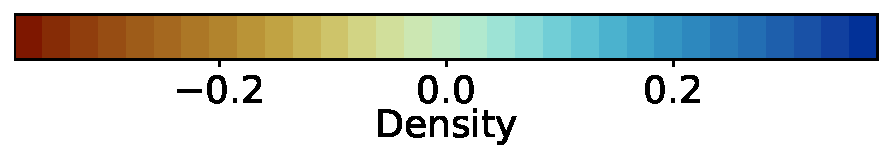
\includegraphics[width=8cm]{./case1/rho_ana_cbhorz.pdf}
	\end{multicols}
	
	\vspace{-0.3in}
	
	\begin{multicols}{4}
		\includegraphics[width=7cm]{./case1/vel_uw.png}\par
		\hspace{0.75in}
		\includegraphics[width=7cm]{./case2/vel_uw.png}\par
		\hspace{1.5in}
		\includegraphics[width=7cm]{./case3/vel_uw.png}\par
		\hspace{2.25in}
		\includegraphics[width=7cm]{./case4/vel_uw.png}
	\end{multicols}
	\vspace{-0.3in}
	\begin{multicols}{4}
		\hspace{0.2in} \includegraphics[width=6cm]{./case1/v_ana_cbhorz.pdf}\par
		\hspace{0.95in} \includegraphics[width=6cm]{./case2/v_ana_cbhorz.pdf}\par
		\hspace{1.8in} \includegraphics[width=6cm]{./case3/v_ana_cbhorz.pdf}\par
		\hspace{2.45in} \includegraphics[width=6cm]{./case4/v_ana_cbhorz.pdf}
	\end{multicols}
	
	\vspace{-0.3in}
	\begin{multicols}{4}
		\includegraphics[width=7cm]{./case1/p_uw.png}\par
		\hspace{0.75in}
		\includegraphics[width=7cm]{./case2/p_uw.png}\par
		\hspace{1.5in}
		\includegraphics[width=7cm]{./case3/p_uw.png}\par
		\hspace{2.25in}
		\includegraphics[width=7cm]{./case4/p_uw.png}
	\end{multicols}
	\vspace{-0.3in}
	\begin{multicols}{4}
		\hspace{0.2in} \includegraphics[width=6cm]{./case1/p_ana_cbhorz.pdf}\par
		\hspace{0.95in} \includegraphics[width=6cm]{./case2/p_ana_cbhorz.pdf}\par
		\hspace{1.8in} \includegraphics[width=6cm]{./case3/p_ana_cbhorz.pdf}\par
		\hspace{2.45in} \includegraphics[width=6cm]{./case4/p_ana_cbhorz.pdf}
	\end{multicols}
	
\end{figure*}


\end{document}